\documentclass[11pt, oneside]{article}   	% use "amsart" instead of "article" for AMSLaTeX format
\usepackage{geometry}                		% See geometry.pdf to learn the layout options. There are lots.
\geometry{letterpaper}                   		% ... or a4paper or a5paper or ... 
%\geometry{landscape}                		% Activate for rotated page geometry
%\usepackage[parfill]{parskip}    		% Activate to begin paragraphs with an empty line rather than an indent
\usepackage{graphicx}				% Use pdf, png, jpg, or eps§ with pdflatex; use eps in DVI mode
								% TeX will automatically convert eps --> pdf in pdflatex	
\usepackage{caption}
\usepackage{subcaption}
\usepackage{float}

\graphicspath{ {./LabReportAssignment1Images/}}	
\usepackage{amssymb}
\usepackage{float}


%SetFonts

%SetFonts


\title{Assignment 4: \\ Twitch Network Analysis}
\author{\centering Ivo L. Arasin (r0926378) \and Vancesca Dinh (r0930510) \and Linas J. Leščinskas (r0874301) \and Yavuz Yavuzhan (r0920104)}
%\date{}							% Activate to display a given date or no date

\begin{document}
\maketitle
\section{Preface}
Twitch offers a pool richly endowed with content wide in breadth and gluttonous in depth. The task at hand is to take on a small sliver of said pool in an open ended analysis. We believe it is useful to put on the goggles of an advertiser looking to place their ads alongside streamers. In this vein, an ensuing analysis is given guardrails and insights can be usefully framed.\newline
The efforts of our analysis mainly focus on clustering streamers and subsequently characterising discovered clusters. Some ideas from the text-mining domain are applied in an effort to describe clusters and unearth some additional insight.
\section{Data}
Since the dataset is rather large, we decided to work on a subset. All streamers with average views of at least 1100 along with their relations and related nodes, i.e. \textit{squads}, \textit{tags} and \textit{games} are kept. The remainder is discarded without further consideration. This results in 4681 streamers, representing a little more than 5\% of the total amount of streamers in the original dataset. From an advertiser's perspective, this is sensible since ads should be placed to those with large audiences. More generally, it is likely that more data would merely corroborate existing, but not bring to light fundamentally new insights (something which we have anecdotally verified but certainly not proven). Furthermore, any attempt to visualize such voluminous data will inevitably result in a clutter that is more artistic than revealing anyway.
\newline
Additionally, we decided to omit \textit{squads} from further analysis too. Inspection of streamers and squads in a network graph shows many microscopic and isolated clusters containing at most a handful of streamers. A few are thinly connected by one streamer belonging to multiple clusters.
Ultimately though, we believe this is not germane to overall clustering efforts.
Next to \textit{squads}, we also only consider \textit{tags} that appear at least ten times.
\newline
Thus our analysis focuses on a dataset that contains 4681 streamers, 2476 games, 1024 tags and 77573 directed relations between them.

\section{Analysis}

To cluster the data, Modularity (in \textit{Gephi} implemented as the Louvain method) is used. It detects 34 clusters. As many of the clusters are rather small, we only consider those with a size of at least 5\% of total streamers (i.e. a cluster should contain at least 234 streamers) for more detailed analysis.
ForceAtlas2 is used for the graph layout.
\newline
It is noteworthy to point out that even though Modularity and the graph layout algorithm of ForeAtlas2 do not communicate with one another, i.e. both methods were executed independently of one another, the visually discernible clusters appear to strongly correlate with the node-color, as determined by Modularity. Thence they complement each other very well.
\subsection{Betweenness}
To enrich the visualization, the betweenness score is calculated (based on \textit{recommends}-relationships) for each streamer and used as the node-size. Larger nodes correspond to nodes with high betweenness. As could be expected, streamers with high betweenness mostly sit at the edge of between clusters, thus acting, in-effect, as a "hub" (c.f. Figure 1).

\subsection{Cluster characterization}
Borrowing a method from text-mining, Latent Dirichlet Allocation (LDA) is applied on a per cluster basis to analyse associated games and tags.
\newline
Each streamer within a cluster is linked to a number of games (or tags). For each cluster, all linked games (or tags) are aggregated and compose the representative vector. This vector is just a long list of all games (or tags) played, where duplicates are of course allowed. Such a representation can be converted into a bag-of-words representation with tuples indicating which game is played and how often it is played (which tag occurs and how frequent it is). Said bag-of-words vector essentially corresponds to a document composed of different words. All clusters together form the corpus.
\newline
LDA is applied individually both on cluster-documents composed of games and on cluster-documents composed of tags. For both, the number of topics is set to 20 (remember, number of clusters is 34) to induce some abstraction and not rely just on a frequency count per cluster (which would be the case if the number of topics was set to 34).
\newline
All clusters are linked to one topic only with a probability of $>$90\%. Figure 2 depicts the clustering along with the clusters' most descriptive games and tags.

\begin{figure}
\centering
	\makebox[\textwidth][c]{\includegraphics[width=1.4\textwidth]{reportImages/graph_wGames_NodeSizes.png}}%
	%\includegraphics[width=1.3\linewidth]{reportImages/graph_wGames_NodeSizes.png}
\caption{Streamers and games in graph network, streamer-node sized based on betweenness}
\label{figure label}
\end{figure}

\begin{figure}
\centering
	\makebox[\textwidth][c]{\includegraphics[width=1.4\textwidth]{reportImages/ClusterFull.png}}%
	%\includegraphics[width=1.3\linewidth]{reportImages/graph_wGames_NodeSizes.png}
\caption{Streamers and games in graph network, enriched with descriptive features: games (bold) and tags}
\label{figure label}
\end{figure}
\subsection{Evaluation}
Above graphs are revealing. As could be expected, a handful of highly popular games dominate all clusters, such as "Just Chatting", "Grand theft Auto V", "VALORANT", "League of Legends" etc. Furthermore, dominant languages such as English can also be found in every cluster.
Still, in spite of this and the notably degree of dispersion of the blue (31) and orange (14) cluster, all clusters are distinct in some way. 
\newline
The green (17) community on top is mainly composed of Russian speakers and popular games are "Dota 2", Virtual Casino" and "Counter Strike: Global Offensive". The dark grey community (20) is composed predominantly of Spanish speakers with the most popular game being "Minecraft" (not considering "Just Chatting" as a game). The ming-green cluster (23) is French in majority and likes to play "Fortnite".
\newline
It is also notable that clusters are differentiated in large part by language, indicating that language is an important feature for Twitch's recommendations. 
\section{Analysis beyond clustering}
\subsection{Random Walk}
To increase an advertisement's chance of success, we hypothesise its placement should aim for consistent engagement on same set of viewers. In other words, an ad should remain highly visible and continuously engage its target audience, instead of trying to reach a maximal number of viewers at any cost.
Since we already have a good clustering, we now try to find some degree of loyalty within a community to determine the tendency of viewers of a community to stick to it and not transition to another one.
If some of the streamers within a community are chosen for an ad, their viewers should actively navigate between other streamers in the community but stay within the circle. For measuring this behavior, we make the following assumption: \textit{Viewers tend to explore other streamers they encounter through recommendations}.
\newline
\newline
We then apply the following methodology:
An adjacency matrix is constructed for every community by aggregating the \textit{recommends} edges. Its values are converted to probabilities by dividing over the row-sum. Markov-chain transitions are applied for 20. for 50 and for 100 iterations. Results are stored as individual retention metrics.
\newline
In a second step, Pagerank is applied for each community to determine the top five streamers. Subsequently, personalized Pagerank is applied to the top five identified streamers with their probabilities being uniform and the probabilities of the remaining streamers outside the top five being set to 0.
Then, personalized Pagerank is applied on the entire graph once more. Intermediate scores of all steps are saved and aggregated per community/cluster to form a measure of retention. When tabulated, interesting insights can be drawn.
\newline
\newline
\textit{Illustrative insights}:
\begin{itemize}
\item \textit{Chess players (community 13)}: even though they are a smaller community, they are closely connected with a random walk retention probability with 0.98. They also have more than 2000 median view count. They are predominantly chess enthusiasts but they also play “Rocket League”. These people also have the tag of “Dead by Daylight”, indicating that they are night owls.
\item \textit{Korean indie-game players (community 15)}: they have the top performance in Markov-chain retention, even in the 100 period case, indicating that they have loyal and closely-knit viewer base. These communities demonstrate relatively lower scores in terms of degree centrality for tags and games, suggesting an inclination towards novelty and a willingness to explore new experiences. Their viewers might be a good fit for a new product launch as a potential of early adopters.
\item \textit{Minecraft and Sports players who are Spanish in majority (community 5)}: they form a community of about 500 streamers and have a random walk retention probability of 0.99 and Markov-chain transition probability of 0.84 in 20 period-case. Their median view-count is a little over 2000. They are also recommended by other communities therefore viewer exposure could be further increased.
\end{itemize}
Such insights can be valuable when wanting to target specific demographics. The three examples above are not exhaustive but give an indication that homogenous communities can be identified in accordance to any advertisement-requirements. A tabular overview can be found in the Appendix.

\subsection{tf-idf}
Although betweenness lends itself quite naturally to a clustering set-up, many other approaches exist. An advertiser might not be interested in the bridge-building behaviour of streamers but in some measure of their uniqueness. We define uniqueness as streamers that are popular (i.e. all those within our subset since they have at least 1100 average views) but do not play generally popular games and are thus catering to a hardened nerd-audience or just happen to dominate some domain of games which other neglect. The concept of tf-idf from text-mining is well suited to represent this metric. If we think of individual games as words and streamers who play those games as composite documents thereof, we can readily apply tf-idf. Those that play games many others are playing too will be punished (inverse-document frequency) whereas those that play games that no-one else is streaming will gain. Streamers who do both will have mid-ranged tf-idf scores (c.f. Figure 3).
\newline
For example, "wolviehd" is streaming a single game and has a high tf-idf score as it is a game no one else is playing. The flock of streamers  streaming only "Just Chatting", which is the overall most popular "game", correspondingly have a minimal tf-idf.
Another case in point is the streamer "gamesdonequick" who streams a large number of games but still has a relatively high tf-idf score, or uniqueness as the games played are almost entirely exclusive to this streamer.
\newline
As an advertiser this property of streamers adds an additional degree of granularity and can be used for specific targeting. An indie-game developer might find it interesting to place ads alongside "gamesdonequick" (in pink cluster 16) due to the streamer's large audience, high degree of differentiation/uniqueness and special focus on unique games, often developed by smaller studios.

\begin{figure}
\centering
	\makebox[\textwidth][c]{\includegraphics[width=1.4\textwidth]{reportImages/graph_tfidf.png}}%
\caption{Streamers and games in graph network, streamer-node sized based on tf-idf}
\label{figure label}
\end{figure}

\section{Concluding remarks}
Our discoveries reveal a good degree of differentiation among clusters. This dissection is insightful from a standpoint of curiosity but becomes actually valuable when inspected from the vantage-point of an advertiser.
Additional measures such as the Random Walk or the tf-idf score equip clusters and streamers with additional nuance.
Ultimately, an exhaustive analysis seems to be out of reach but was not the aim of us anyway. However, the data undoubtedly still holds much more that what we have brought to light which is why we loosely framed our analysis from the perspective of an advertiser to make sense of findings and direct our efforts broadly in one consistent direction.
\clearpage

\section{Appendix}
Data used throughout the analysis and for visualization purposes.
\begin{figure}[H]
\centering
	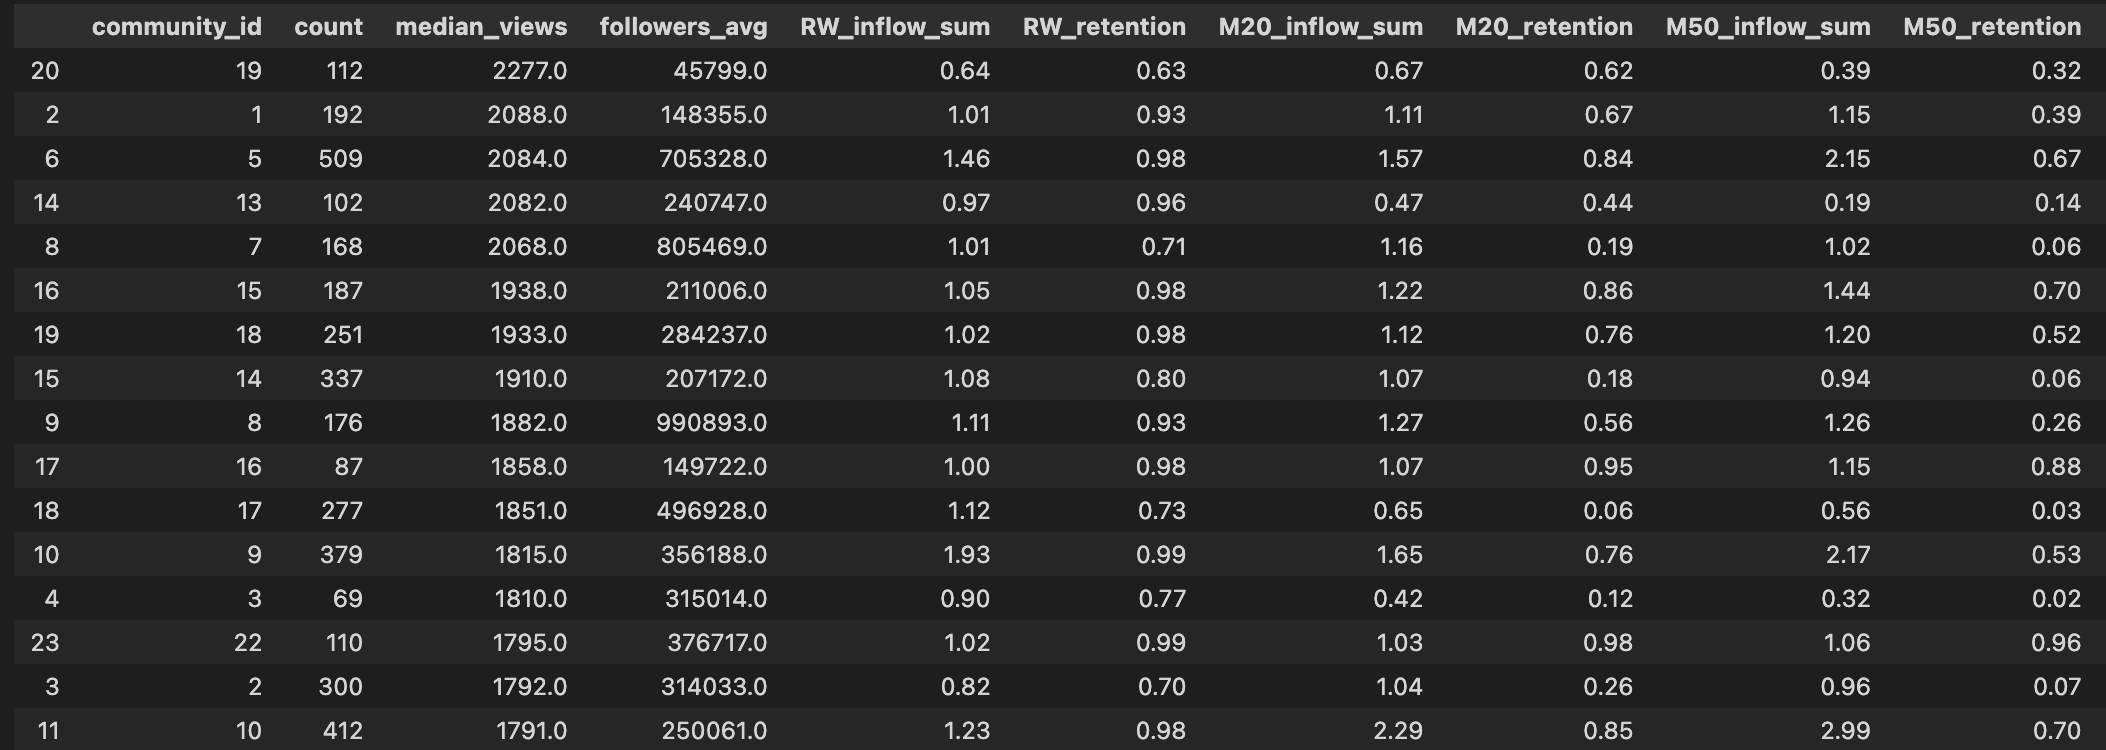
\includegraphics[width=1\linewidth]{reportImages/Yavuz_table.png}
\caption{Table of results of Random Walk segment}
\label{figure label}
\end{figure}

\begin{table}[H]
\caption {top 10 streamers by betweenness} 
    \centering
    \begin{tabular}{|l|l|l|l|l|}
    \hline
        \textbf{name} & \textbf{views\_avg} & \textbf{tfidf\_score} & \textbf{betweenness} & \textbf{clusterID} \\ \hline
        esl\_csgo & 15028 & 0.015643275 & 0.06843872629380872 & 15  \\ \hline
        shroud & 17814 & 0.119327649 & 0.04027987787945484 & 16  \\ \hline
        xqc & 57999 & 0.091482006 & 0.040069984361607754 & 16  \\ \hline
        otplol\_ & 9533 & 0.001890359 & 0.034243000548030755 & 23  \\ \hline
        foolish\_gamers & 6988 & 0.158491572 & 0.03248278489686211 & 20  \\ \hline
        krl\_stream & 1301 & 0.003508772 & 0.032289837468070376 & 15  \\ \hline
        summit1g & 17310 & 0.100935789 & 0.03152296828251939 & 16  \\ \hline
        kaicenat & 57645 & 0.065497628 & 0.02828144371874025 & 31  \\ \hline
        place & 2295 & 0.004150845 & 0.02795975287638164 & 17  \\ \hline
        aspaszin & 10992 & 0.001912046 & 0.0260724840101937 & 31 \\ \hline
    \end{tabular}
\end{table}

\begin{table}[H]
\caption {top 10 streamers by tf-idf}
    \centering
    \begin{tabular}{|l|l|l|l|l|}
    \hline
        \textbf{name} & \textbf{views\_avg} & \textbf{tfidf\_score} & \textbf{betweenness} & \textbf{clusterID} \\ \hline
        ai\_sponge & 6768 & 1 & 0.001080759702814037 & 16  \\ \hline
        skzlatamproject & 5979 & 1 & 0.0 & 12  \\ \hline
        pronewstv & 1584 & 1 & 0.0 & 24  \\ \hline
        juliapitzer & 2474 & 1 & 0.0 & 18  \\ \hline
        joltzdude139 & 1224 & 1 & 0.0 & 21  \\ \hline
        himetokki & 1597 & 1 & 0.0 & 25  \\ \hline
        oreitroll & 2155 & 1 & 0.0 & 26  \\ \hline
        superzomgbbq & 1646 & 1 & 0.0 & 28  \\ \hline
        ruwarface & 1941 & 1 & 0.0 & 17  \\ \hline
        wolviehd & 1259 & 1 & 0.0 & 20 \\ \hline
    \end{tabular}
\end{table}
\begin{table}[H]
\caption {top 10 streamers by avg. views} 
    \centering
    \begin{tabular}{|l|l|l|l|l|}
    \hline
        \textbf{name} & \textbf{views\_avg} & \textbf{tfidf\_score} & \textbf{betweenness} & \textbf{clusterID} \\ \hline
        kingsleague & 304985 & 0.007575758 & 2,54E+12 & 20  \\ \hline
        evelone192 & 91097 & 0.002029262 & 5,19E+11 & 17  \\ \hline
        thegrefg & 83245 & 0.005539516 & 0.00142583721354589 & 20  \\ \hline
        austinshow & 80671 & 0.000549753 & 0.0 & 16  \\ \hline
        auronplay & 80200 & 0.073886222 & 7,40E+11 & 20  \\ \hline
        ibai & 78567 & 0.004991274 & 0.0032769028420825217 & 20  \\ \hline
        paulinholokobr & 78441 & 0.067664913 & 1,33E+12 & 31  \\ \hline
        elspreen & 78124 & 0.035979881 & 0.003024240390287704 & 20  \\ \hline
        adinross & 73424 & 0.00149737 & 6,47E+10 & 31  \\ \hline
        asmongold & 66555 & 0.009708738 & 0.0 & 29 \\ \hline
    \end{tabular}
\end{table}





\end{document}  
